\documentclass[11pt]{article}
\usepackage[a4paper,left=20mm,top=10mm,right=20mm]{geometry}
\usepackage[OT2]{fontenc}
\usepackage{graphicx}
\pagenumbering{gobble}
\usepackage{amsfonts}
\usepackage{amsthm}
\usepackage{amsmath}
\newcommand\tsd{\theoremstyle{definition}}
\newcommand\tsr{\theoremstyle{remark}}

\newcommand\eng{\fontencoding{OT1}\fontfamily{\rmdefault}\selectfont}
\newcommand\srb{\fontencoding{OT2}\fontfamily{\rmdefault}\selectfont}

\title{\bf{Kvantni kompas}}
\author{\Large Aleksa Vuchkovic1, 2c}
\date{}

\begin{document}
\maketitle
\Large\noindent
Evolucija je otkrila kvantna dejstva mnogo pre nego shto su nauchici uopshte i posumnjali u njihovo postojanje i iskoristila ih da zhiva bic1a opremi kompletom velichanstvenih sposobnosti: moguc1nosh${}$c1u sprovodjenja fotosinteze, prepoznavanje smera magnetnog polja, a danas nauchnici istrazhuju moguc1nost da mozhda chak i nasha svest postoji i radi zahvaljujuc1i upravo kvantnim pojavama.\\
Pricha koja se meni najvishe dopala je o magnetnom kompasu crvendac1a.\\
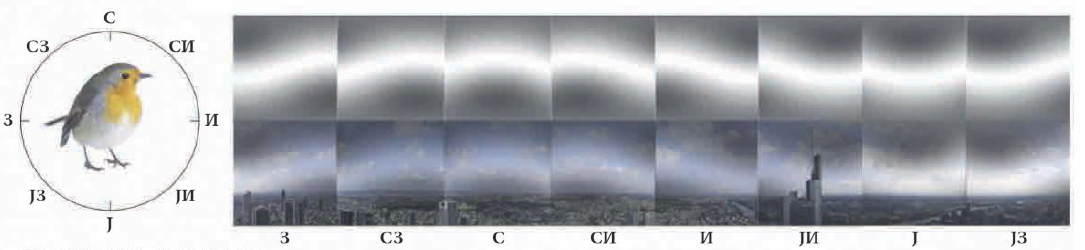
\includegraphics[scale=0.8]{Capture}
Rozvita i Volfgang Vilchko dokazali su sedamdesetih godina proshlog veka da ptice mogu da osete magnetno polje planete, a danas fizichari detaljno istrazhuju magnetni kompas u oku crvendac1a koji mozhe da otkrije nagib linija Zemljinog magnetnog polja u odnosu na povrshinu planete. Na slici je prikazan primer vizuelnog opazhanja Frankfurta na Majni sa visine od 200m koji ima ova ptica i moguc1nost razlikovanja smerova kretanja od polozhaja linija magnetnog polja koje se prostiru pod uglom od 66 stepeni.\\
\end{document}